\documentclass[class=scrartcl, crop=false]{standalone}

\usepackage[sexy]{/home/gautierk/.config/evan}
\usepackage{/home/gautierk/.config/Latex/cole}

\date{2019-11-15}


\begin{document}

\section{Tutorial 11-15}

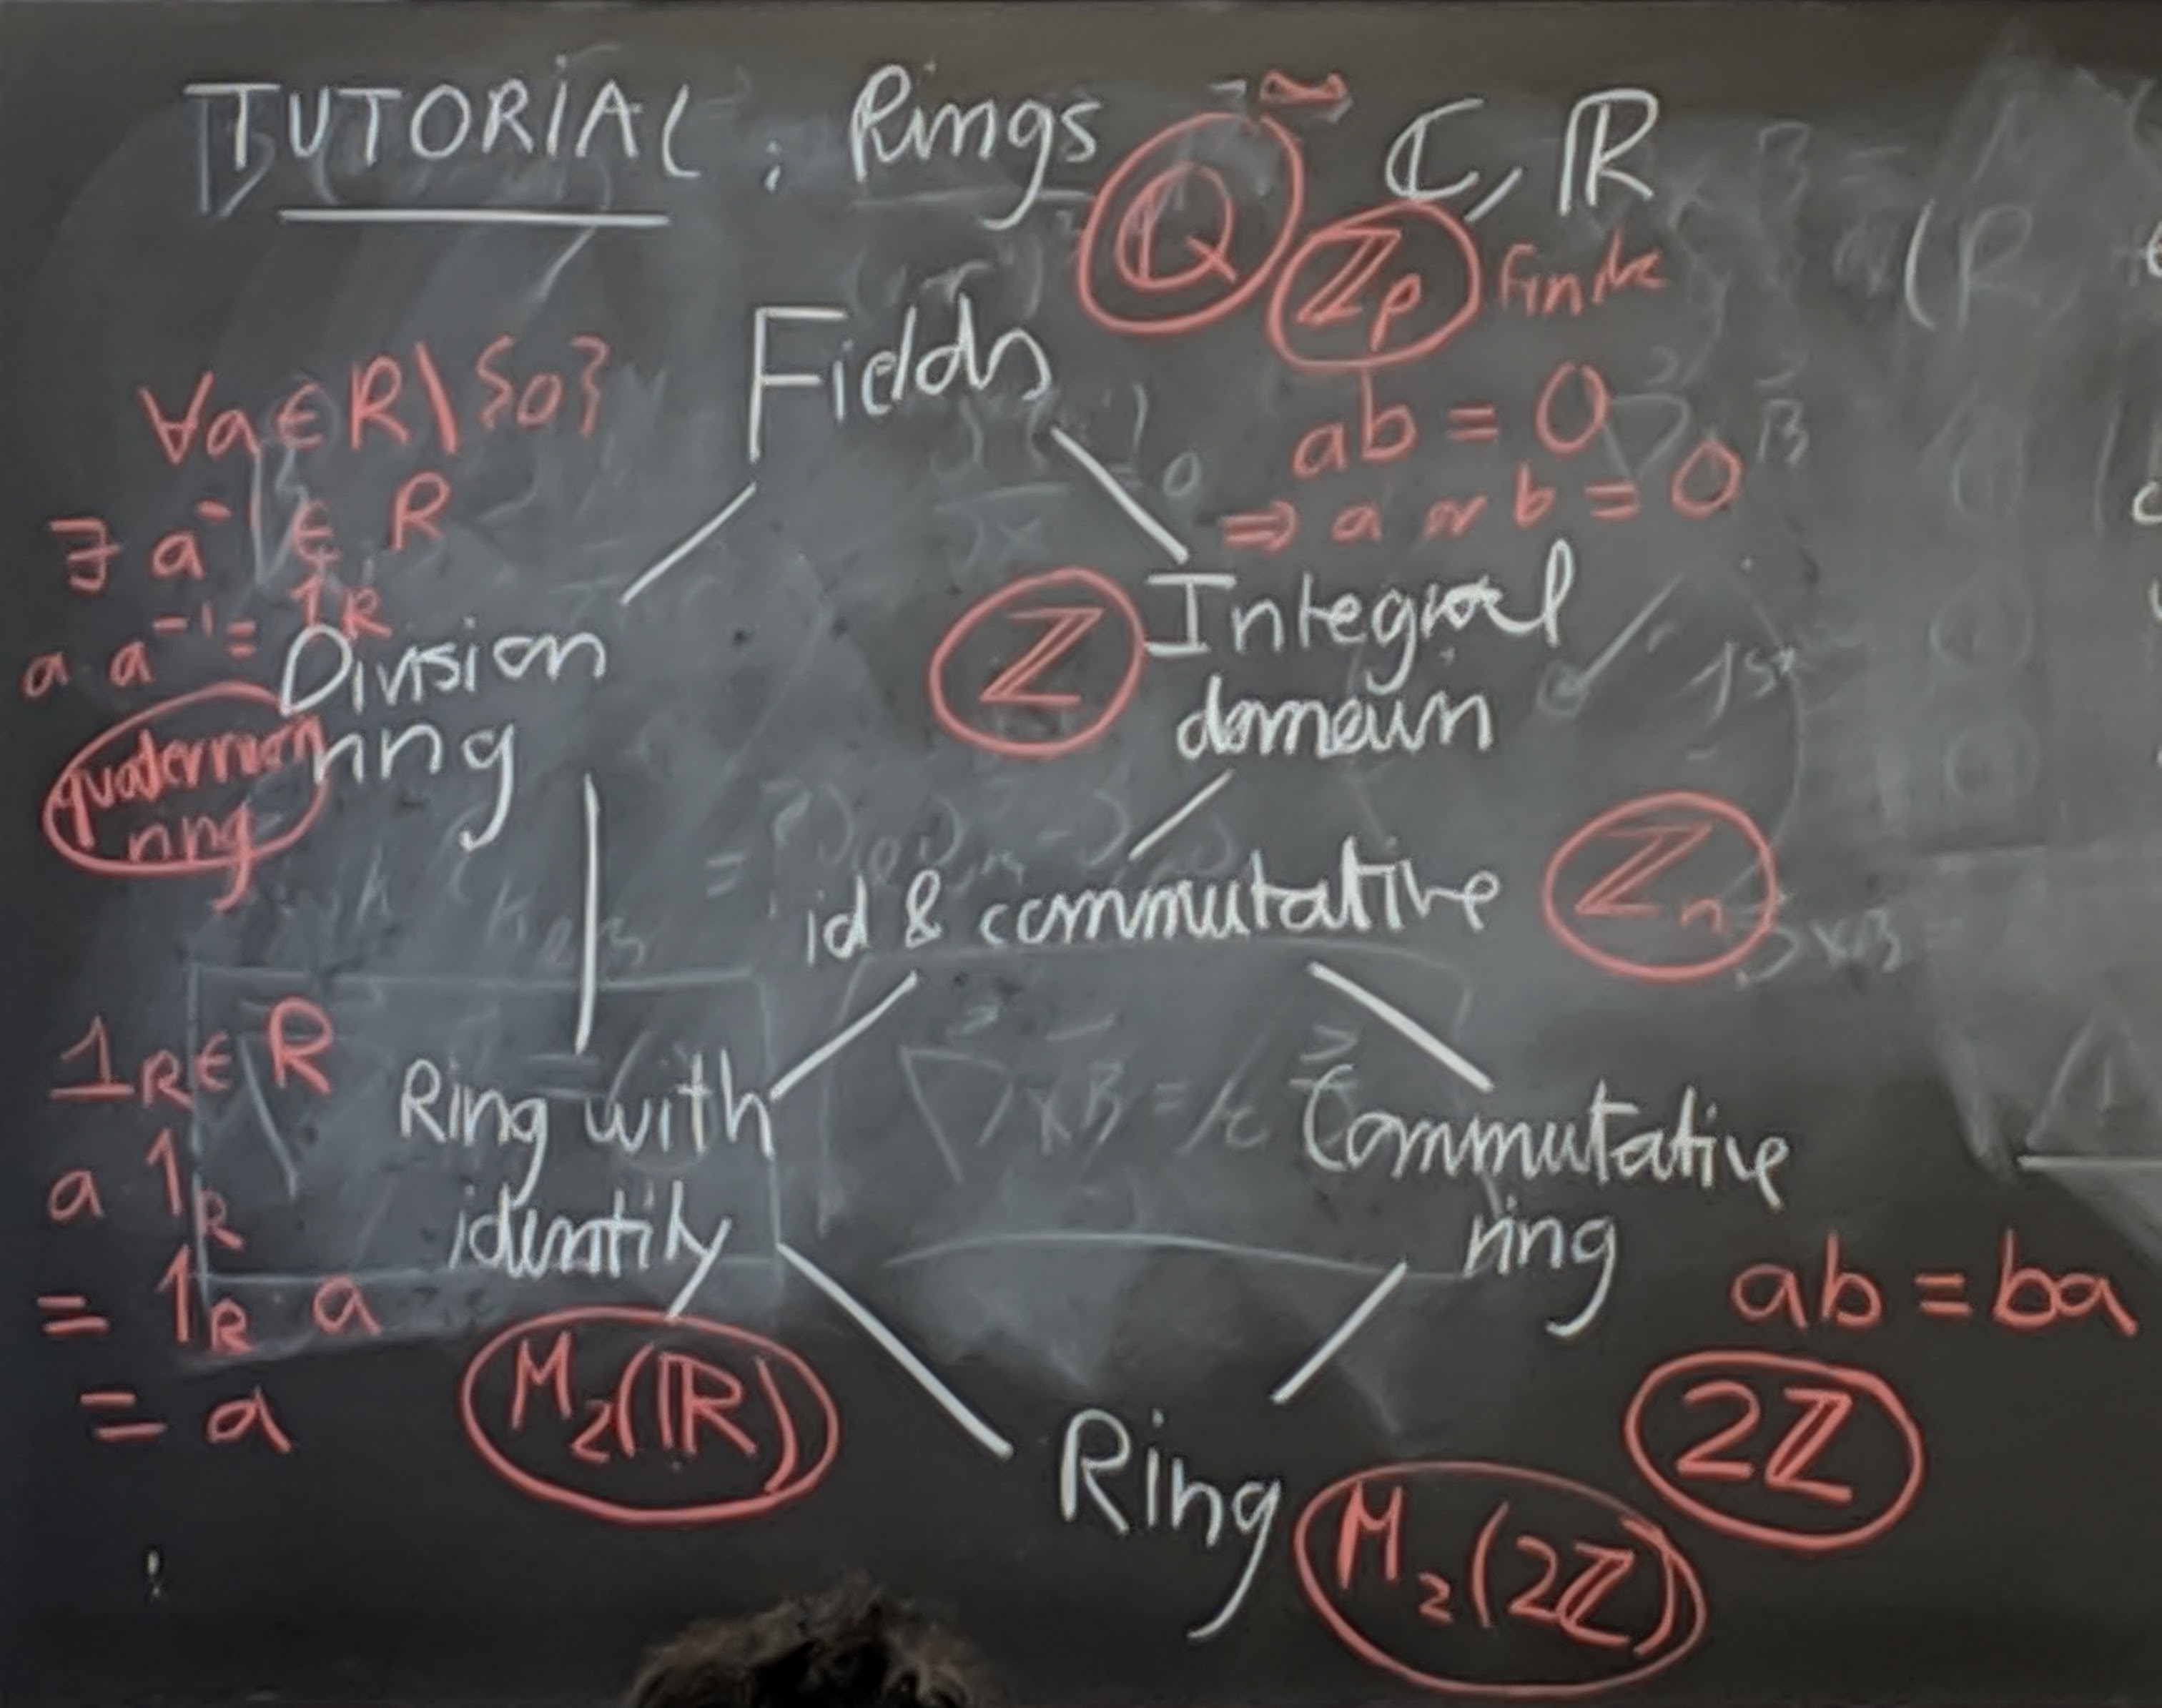
\includegraphics[width=\textwidth]{/home/gautierk/McGill/235math/notes/lectures/images/ring_fields_diagram.jpg}

\begin{definition}
  $(R, + , \cdot)$ is a ring if
  \begin{enumerate}
    \ii $(R, +)$ is an abelian group.
    \ii $(ab)c = a(bc)$.
    \ii $a(b + c) = ab + ac$ and $(a + b)c = ac + bc$.
  \end{enumerate} 
\end{definition} 

Caution: $(R, \cdot)$ is not a group.

\begin{example}
  $(\ZZ, +, \cdot)$ is a ring.
  \begin{enumerate}
    \ii $(\ZZ, +)$ is an abelian group.
    \ii 2 is satisfied.
    \ii 3 is satisfied.
  \end{enumerate} 
\end{example} 
\begin{example}
  $(\ZZ, \cdot)$ is not a group because $\forall n \in \ZZ$, $n \neq 1, -1$, then $\not\exists n^{-1} \in \ZZ$.
\end{example} 

\begin{exercise}
  Find an example for each type of ring.

  \begin{enumerate}
    \ii Ring: $M_2(2\ZZ)$ doesn't have the identity and isn't commutative.
    \ii Ring with Identity: $M_2(\RR)$. Matrix multiplication is not commutative but $M_2(\RR)$ contains the identity element.
    \ii Commutative Ring: $2\ZZ$. Commutative, but doesn't contain the multiplicative identity element.
    \ii Division Ring: Quaternion Ring
    \ii Identity and Commutative: $\ZZ_n$ where $n$ is not prime. It has the identity and multiplication is commutative, but it is not an integral domain.
    \begin{gather*}
      a, b \in \ZZ_n \ \text{where} \ n = ab \\
      \Rightarrow a \cdot b = 0 \mod(n)
    \end{gather*} but $a, b \neq 0$.
    \ii Integral Domain: $\ZZ$ because there is identity, multiplication is commutative, there aren't any zero divisors, but there aren't inverses for all elements.
    \ii Field: Examples include $\QQ$ and $\ZZ_p$ where $p$ is prime.
  \end{enumerate} 
\end{exercise} 

\begin{example}
  Let $R$ be a ring. $x \in R$ is idempotent if $x^2 = x$. Show that the only idempotent elements in an integral domain are $0$ and $1$.
  \\\\
  Let $x \in \RR$, where $R$ is an integral domain, such that $x^2 = x$.
  \begin{gather*}
    x^2 = x \\
    \Rightarrow x^2 - x = 0 \\
    \Rightarrow x(x - 1) = 0 \\
    \text{Because $R$ is an integral domain, this implies that} \ x = 0 \ \text{or} \  x = 1
  \end{gather*} 
  Note that the following argument would be incorrect because $R$ is not a division ring:
  \begin{gather*}
    x \neq 0 \\ 
    \Rightarrow x^{-1} x^2 = x^{-1} x \\
    \Rightarrow x = 1
  \end{gather*} 
\end{example} 

\begin{theorem}
  Let $R$ be an integral domain. Then $ab = ac \Rightarrow b = c$.
  \begin{example}
    In $\ZZ$ (an integral domain):
    \begin{gather*}
      n \cdot m = n \cdot m' \\
      \Rightarrow m = m'
    \end{gather*} 
    In $\ZZ_6$ (not an integral domain): 
    \begin{gather*}
      3 \cdot 2 = 3 \cdot 4 = 0
    \end{gather*} but 2 is not equal to 4.
  \end{example} 
\end{theorem} 

\begin{example}
  Prove or disprove: $R$ is a ring with identity $1_R$. $S \subset R$ is a subring that has identity $1_S$. Then does $1_R = 1_S$?
  \\\\
  FALSE. Counter example:
  \\\\
  $R = \ZZ_6$ ring with identity $1_R = 1$ and $S = \{0, 3\}$.
  \\\\
  Subring conditions:
  \begin{enumerate}
    \ii $S \neq \varnothing$ 
    \ii $r - s \in S$ $\forall r, s \in S$ 
    \begin{gather*}
      0 - 0 = 0 \in \ZZ_6 \\
      0 - 3 = 3 \in \ZZ_6 \\
      3 = 3 = 0 \in \ZZ_6
    \end{gather*} 
    \ii $r \cdot s \in \S \ \forall r, s \in S$
     \begin{gather*}
      0 \cdot 0 = 0 \in \ZZ_6 \\
      0 \cdot 3 = 0 \in \ZZ_6 \\
      3 \cdot 3 = 3 \in \ZZ_6
    \end{gather*}
  \end{enumerate} 
  But $1_R = 1 \neq 3 = 1_S$.
\end{example} 

\begin{example}
  Is $\ZZ[i] = \{a + bi \ | \ a, b \in\ZZ\}$ an integral domain?
  \begin{enumerate}
    \ii Ring $\checkmark$ 
    \ii Identity $1 \ \checkmark$ 
    \ii Commutative $\checkmark$ 
    \begin{gather*}
      (a + bi)(c + di) = (ac - bd) + (ad + bc)i = (c + di)(a + bi)
    \end{gather*} 
    Follows because addition and multiplication in $\ZZ$ are commutative .
    \ii No zero divisors:
    \begin{gather*}
      \text{Assume } a + bi \neq 0 \\
      (a + bi)(c + di) = 0 \\
      \Rightarrow (a - bi)(a + bi)(c + di) \\
      \Rightarrow \underbrace{(a^2 + b^2)}_{\in \ZZ}(c + di) \\
      \text{Let} \ n = a^2 + b^2 \in \ZZ \\
      \Rightarrow n(c + di) = 0 \\
      \Rightarrow nc + ndi = 0 \\
      \Rightarrow
      \begin{cases}
        nc = 0 \\
        nd = 0
      \end{cases} \Rightarrow c = d = 0 \ \text{because} \ \ZZ \ \text{is an integral domain} \ 
      \\
      \Rightarrow c + di = 0
    \end{gather*} 
    Therefore there are no zero divisors because the only way to satisfy the equality is if $(c + di) = 0$.
  \end{enumerate} 
\end{example} 

\begin{definition}[Ring homomorphism]
  Ring homomorphism: Let $\varphi: R \to S$ where $R, S$ are rings. Then:
  \begin{gather*}
    \varphi(a + b) = \varphi(a) + \varphi(b) \\
    \varphi(ab) = \varphi(a) \varphi(b)
  \end{gather*} 
\end{definition} 

\begin{definition}[Ideal]
  Let $I \subset R$. $I$ is an ideal if it is a subring such that $\forall r \in R$, $rI \subset I$ and $Ir \subset I$.
  \\\\
  i.e. $\forall a \in I$, $\forall r \in R$, $ar \in I$ and $ra \in I$.
\end{definition} 

\begin{example}
  Find all possible ring homomorphisms $\varphi: \ZZ_6 \to \ZZ_{15}$. 
  \\\\
  First we will answer the following: what are all the possible group homomorphisms?
  \\\\
  $\ZZ_6 = \langle 1 \rangle $ is cyclic so $\varphi$ is defined by $\varphi(1)$. i.e.
  \begin{gather*}
    1 \to x \\
    \Rightarrow n \to nx
  \end{gather*} 
  Also, 
  \begin{gather*}
    0 = \varphi(0) = \varphi(6) = 6x \in \ZZ_{15} \\
    \Rightarrow [6x]_{15} = 0 \\
    \Rightarrow [2x]_5 = 0 \\
    \Rightarrow [x]_5 = 0
  \end{gather*} 
  So the possible values of $x$ are $x = \{0, 5, 10\}$. Group homomorphisms: 
  \begin{gather*}
    \varphi_0: 1 \to 0 \\
    \varphi_5: 1 \to 5 \\
    \varphi_{10}: 1 \to 10
  \end{gather*} 
  Are these also ring homomorphisms?
  \begin{enumerate}
    \ii $\varphi_0$. $\checkmark$
    \begin{gather*}
      1 \to 0 \\
      n \to 0 \\
      \varphi(nm) = nm \cdot 0 = 0 \varphi(n)\varphi(m)
    \end{gather*} 
      \ii $\varphi_5$ 
      \begin{gather*}
        1 \to 5 \\
        n \to 5n \\
        \varphi(nm) = 5 nm \\
        \varphi(n) \varphi(m) = 5n \cdot 5m = 25 nm = 10nm \\
        5 nm \neq 10 nm \ \text{so not a ring homomorphism} \ 
      \end{gather*} 
      \ii $\varphi_{10}$. $\checkmark$
      \begin{gather*}
        1 \to 10 \\
        n \to 10n \\
        \varphi(nm) = 10nm \\
        \varphi(n) \varphi(m) = 10 n \cdot 10m = 100 nm = 10 nm
      \end{gather*} 
  \end{enumerate} 
  So the ring homomorphisms from $\ZZ_6 \to \ZZ_{15}$ can be described by $\varphi(1) = 0$ and $\varphi(1) = 10$.
\end{example} 


\end{document}
